\DiaryEntry{Legendre Polynomials - Generating Function}{2018-09-18}{Maths}

We start with the electrostatic potential of a single charge $q$ which we want to express in polar coordinates. The charge is displaced by $a$ to the right from the origin; see Figure below.


\begin{figure}[H]
	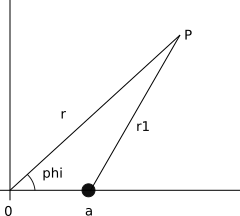
\includegraphics[scale=1.0]{images/legendre_dipol.png}
\end{figure}

The potential $\phi$ is given by

\bee
\Phi = \frac{q}{4\pi\epsilon_0} \frac{1}{r_1} = \frac{q}{4\pi\epsilon_0} \frac{1}{\sqrt{a^2 + r^2 - 2ar\cos \phi}}
\eee

where we have used the law of cosine: $r_1^2 = r^2 + a^2 - 2ar\cos\phi$. We can rearrange this in terms of $a/r$ as follows

\bee
\Phi = \frac{q}{4\pi\epsilon_0 r} \frac{1}{\sqrt{1 + \frac{a^2}{r^2} - 2 \frac{a}{r}\cos \phi}}
\eee

Now we make a series expansion in terms of $a/r$ and obtain

\bee
\Phi = \frac{q}{4\pi\epsilon_0 r} \left( 1 + \cos\phi \frac{a}{r} + \frac{3 \cos^2\phi - 1}{2} \left( \frac{a}{r}\right)^2 + \frac{5 \cos^3\phi - 3\cos\phi}{2} \left( \frac{a}{r}\right)^3 + \cdots \right)
\eee

The series coefficients are the Legendre Polynomials evaluated at $\cos\phi$; i.e. we can write

\bee
\Phi = \frac{q}{4\pi\epsilon_0 r} \sum_{n=0}^\infty P_n(\cos\phi) \left( \frac{a}{r} \right)^n
\eee

For $r \gg a$ (i.e. for away from the charge), the first few terms will suffice.

Moving away from physics, we can drop all constants, and rename variables to arrive at

\be\label{2018-09-18:eq1}
g(t,x) = \frac{1}{\sqrt{1-2xt+t^2}} = \sum_{n=0}^\infty P_n(x) t^n
\ee

which is the ``generating function formula''.

Let's extend above setting by placing a second charge with charge $-q$ at position $-a$ and calculate the potential

\bee
\Phi = \frac{q}{4\pi\epsilon_0 r} \left( \frac{1}{\sqrt{1 + \frac{a^2}{r^2} - 2 \frac{a}{r}\cos \phi}} - \frac{1}{\sqrt{1 + \frac{a^2}{r^2} + 2 \frac{a}{r}\cos \phi}} \right)
\eee

We can make a series expansion to better see what's going on

\begin{align*}
  \Phi &= \frac{q}{4\pi\epsilon_0 r} \left( \sum_{n=0}^\infty P_n(\cos\phi)\left(\frac{a}{r} \right)^n - \sum_{n=0}^\infty P_n(\cos\phi) (-1)^n \left(\frac{a}{r} \right)^n \right) \\
  &= \frac{2q}{4\pi\epsilon_0 r} \sum_{n=1,3,5,\ldots}^\infty P_n(\cos\phi)\left(\frac{a}{r} \right)^n
\end{align*}

The terms for $n$ being even cancel each other and the odd ones remain. From a physical point of view, the total charge is zero, therefore the $n=0$ term vanishes.

As a first approximation, we have

\bee
\Phi = \frac{2q}{4\pi\epsilon_0 r} P_1(\cos\phi) \frac{a}{r} = \frac{2aq}{4\pi\epsilon_0 r^2} \cos\phi
\eee

where $2aq$ is the dipole moment.


\subsection{Legendre Polynomals recursive definition - Generating Function}

\href{https://math.stackexchange.com/questions/1611224/calculating-i-int-11-dfrac1-sqrt1-xp-nx-dx-where-p-n-is-a?rq=1}{From here}). Let's start with the recursive definition of the Legendre Polynomials,

\bee
(n+1)P_{n+1}(x) = (2n+1)xP_n (x) - nP_{n-1}(x)
\eee

Multiply this definition with $t^{n+1}$ and sum over $n=1,2,3,\ldots$ to obtain

\bee
\sum_{n=1,2,\ldots} t^{n+1}(n+1)P_{n+1} = \sum_{n=1,2,\ldots} t^{n+1}(2n+1)xP_n -\sum_{n=1,2,\ldots} t^{n+1} nP_{n-1}
\eee

The goal is to have sum expressions of the form $\sum_{n=0}^\infty P_n$. The first term can be rewritten

\bee
\sum_{n=1,2,\ldots} t^{n+1}(n+1)P_{n+1} = 2 t^2 P_2 + 3 t^3 P_3 + \cdots = \sum_{n=0}^\infty t^n n P_n - t P_1 = \sum_{n=0}^\infty t^n n P_n - tx
\eee

where we have used the initial condition $P_1 = x$. The second term becomes

\bee
\sum_{n=1,2,\ldots} t^{n+1}(2n+1)xP_n = \sum_{n=0}^\infty t^{n+1}(2n+1)xP_n - t x P_0 = \sum_{n=0}^\infty t^{n+1}(2n+1)xP_n - t x
\eee

with initial condition $P_0 = 1$. The last term is rewritten as

\bee
\sum_{n=1,2,\ldots} t^{n+1} nP_{n-1} = 1 t^2 P_0 + 2t^3 P_1 + 3t^4 P_2 + \cdots = \sum_{n=0}^\infty (n+1) t^{n+2} P_n
\eee

We therefore obtain (with the simplification $\sum_{n=0}^\infty = \sum_n$)

\bee
\sum_{n=0}^\infty n t^n P_n = \sum_n 2 n x t^{n+1} P_n + \sum_n x t^{n+1} P_n - \sum_n n t^{n+2} P_n - \sum_n t^{n+2} P_n
\eee

We have two different ``term types'': One of the form $\sum_n t^n P_n$ and one of the form $\sum_n n t^n P_n$ - the latter can be expressed as derivative of the first one (see further below). We therefore separate expressions along this line and obtain

\bee
(1 - 2xt + t^2) \sum_n n t^n P_n = (tx - t^2) \sum_n t^n P_n
\eee

which we can simplify to

\bee
(1 - 2xt + t^2) \sum_n n t^{n-1} P_n = (x - t) \sum_n t^n P_n
\eee

What we actually seek is an expression for $g(t,x) = \sum_n P_n t^n$. We notice that $g'(t,x) = \frac{\partial g(t,x)}{\partial t} = \sum_n n t^{n-1} P_n$ and above expression therefore is

\bee
(1 - 2xt + t^2) g'(t,x) = (x - t) g(t,x) \rightarrow g'(t,x) = \frac{x-t}{1-2xt+t^2} g(t,x)
\eee

This is a first oder ODE which we can solve according to

\bee
g(t,x) = \exp \left( \int_0^t \frac{x-t'}{1-2xt'+t'^2} \right)
\eee

In order to solve the integral, we substitute $u = 1-2xt'+t'^2, \frac{du}{dt'} = -2x+2t' = (-2(t'-x), dt' = \frac{du}{-2(x-t')}$ and obtain

\bee
\int_0^t \frac{x-t'}{1-2xt'+t'^2} = \int \frac{x-t'}{u}\frac{du}{-2(x-t')} = -\frac{1}{2} \ln u = - \frac{1}{2} \ln \left. \left( 1-2xt' + t'^2 \right) \right|_{t'=0}^t = \ln \frac{1}{\sqrt{1-2xt+t^2}}
\eee

Then, finally, the generating function becomes

\bee
g(t,x) = \exp \ln \frac{1}{\sqrt{1-2xt+t^2}} = \frac{1}{\sqrt{1-2xt+t^2}} \qed
\eee

Note / remark: We are calculating the generating function from a recurrence relation (there are several articles in this journal for this topic). When expressions of the form $P_{n+1}$ or $P_{n-1}$ are included, then the initial conditions $P_0, P_1, \ldots$ may show up. In this case, luckily, the terms involving the initial conditions cancelled; had they not, the ODE for the generating function would have been more complex to solve (if solvable at all). But the principle of solving for the generating function does not depend on the vanishing of these terms.


\paragraph{Application.} We can use the series expansion to integrate some fun looking integrals (based on \href{https://math.stackexchange.com/questions/1611224/calculating-i-int-11-dfrac1-sqrt1-xp-nx-dx-where-p-n-is-a?rq=1}{here}).

\bee
I = \int_{-1}^1 \frac{1}{\sqrt{1-x}} P_n(x) dx
\eee

Let's write down the generating function \eqref{2018-09-18:eq1} again,

\bee
g(t,x) = \frac{1}{\sqrt{1-2xt+t^2}} = \sum_{n=0}^\infty P_n(x) t^n
\eee

which becomes for $t=1$

\bee
g(t=1, x) = \frac{1}{\sqrt{1-2x+2}} = \frac{1}{\sqrt{2}} \frac{1}{\sqrt{1-x}} = \sum_{n=0}^\infty P_n(x)
\eee

and we have

\bee
\frac{1}{\sqrt{1-x}} = \sqrt{2} \sum_{n=0}^\infty P_n(x)
\eee

We can use this series expansion to rewrite the integrand as follows

\bee
I = \sqrt{2} \int_{-1}^1 \left( \sum_{m=0}^\infty P_m(x) \right) P_n(x) dx
\eee

Using the orthogonality of the Legendre Polynomials, we obtain

\bee
I = \sqrt{2} \int_{-1}^1 P_n^2(x) dx = \frac{2\sqrt{2}}{2n+1}
\eee



%%% Local Variables:
%%% mode: latex
%%% TeX-master: "journal"
%%% End:
